\documentclass{standalone}

\usepackage{tikz}
\usepackage{pgf-umlcd}
\usepackage[bitstream-charter]{mathdesign} % +1! taules mes petites i hi caben
\usepackage[T1]{fontenc}
\usepackage[utf8]{inputenc}

\begin{document}

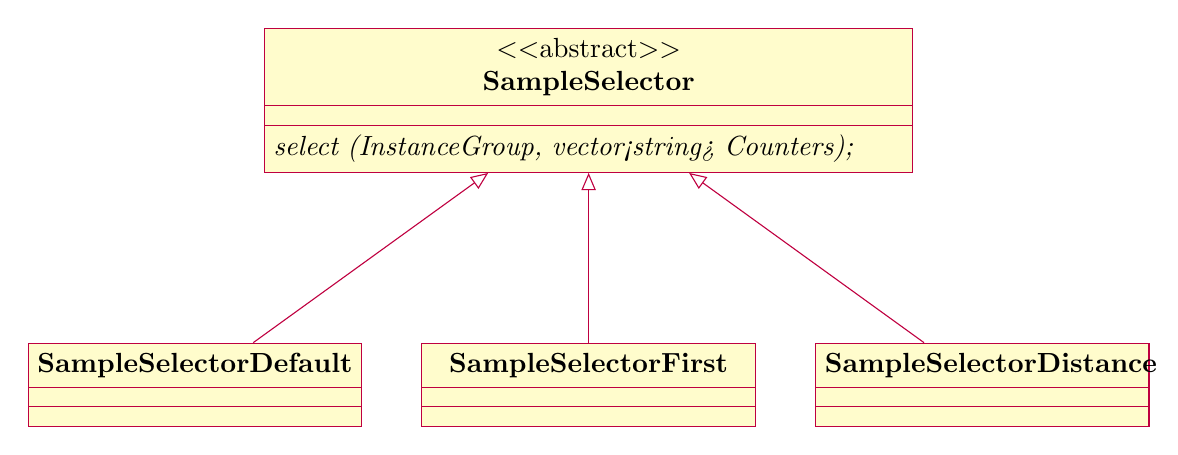
\begin{tikzpicture}

\begin{abstractclass}[text width=8cm]{SampleSelector}{0,0}
\operation[0]{select (InstanceGroup, vector<string> Counters);}
\end{abstractclass}

\begin{class}[text width=4cm]{SampleSelectorDefault}{-5,-4}
\inherit{SampleSelector}
\end{class}
\begin{class}[text width=4cm]{SampleSelectorFirst}{0,-4}
\inherit{SampleSelector}
\end{class}
\begin{class}[text width=4cm]{SampleSelectorDistance}{5,-4}
\inherit{SampleSelector}
\end{class}
\end{tikzpicture}

\end{document}
